
\section{Team}
\label{sec:team}

We are a team of five undergraduate students of the Freie Universität Berlin\link{http://www.fu-berlin.de}{Homepage of Freie Universität Berlin}. Even though we are all in the same year our knowledge regarding the creation of software and the used technologies varied widely. We were however all inexperienced in project management. Specifically none of us had been part of a software development process before. We choose the team name \emph{Scetris}. \emph{Scetris} is an artifical word composed of scheduling and Tetris -- scheduler because of the project itself and Tetris because of the idea of arranging courses in the timetable in way to remove unneccesary space. The members of the team, their age and their most prominent task are:

\begin{description}
	\item[David Bialik] (23) is responsible for the maintenance of the technical aspects of our developing process. He created our ant-based build system and an automated installer that sets up the database and a webserver. He also kept an eye on documentation and unit testing.
	\item[Julian Fleischer] (23) is an enthusiast regarding everything that has to do with programming languages and the semantics of data. As advanced studies he attended a course on XML technologies. He specified and implemented an XML-based format for the creation of object-relation models, from which custom code can automatically be generated. The data access layer, as part of the backend of our application, has emerged that way, as have large parts of the web forms.
	\item[Hagen Mahnke] (24), interested in database technologies developed in pair programming with Konrad the initial scheduler algorithm. Further he has been the communicator for the team.
	\item[Konrad Reiche] (22), whose primary interest lies in algorithms and their efficient implementation, designed and implemented together with Hagen the scheduling algorithm. It works both as a stand alone application as well as an integrated component.
	\item[André Zoufahl] (22) is working part time in a company doing web development, thus he is experienced in the usage of HTML, CSS and accompanying web frameworks. One of his major interests is the visualization of data, thus he was primarily responsible for the development of our user interface. 
\end{description}


\begin{figure}[H]
	\centering
		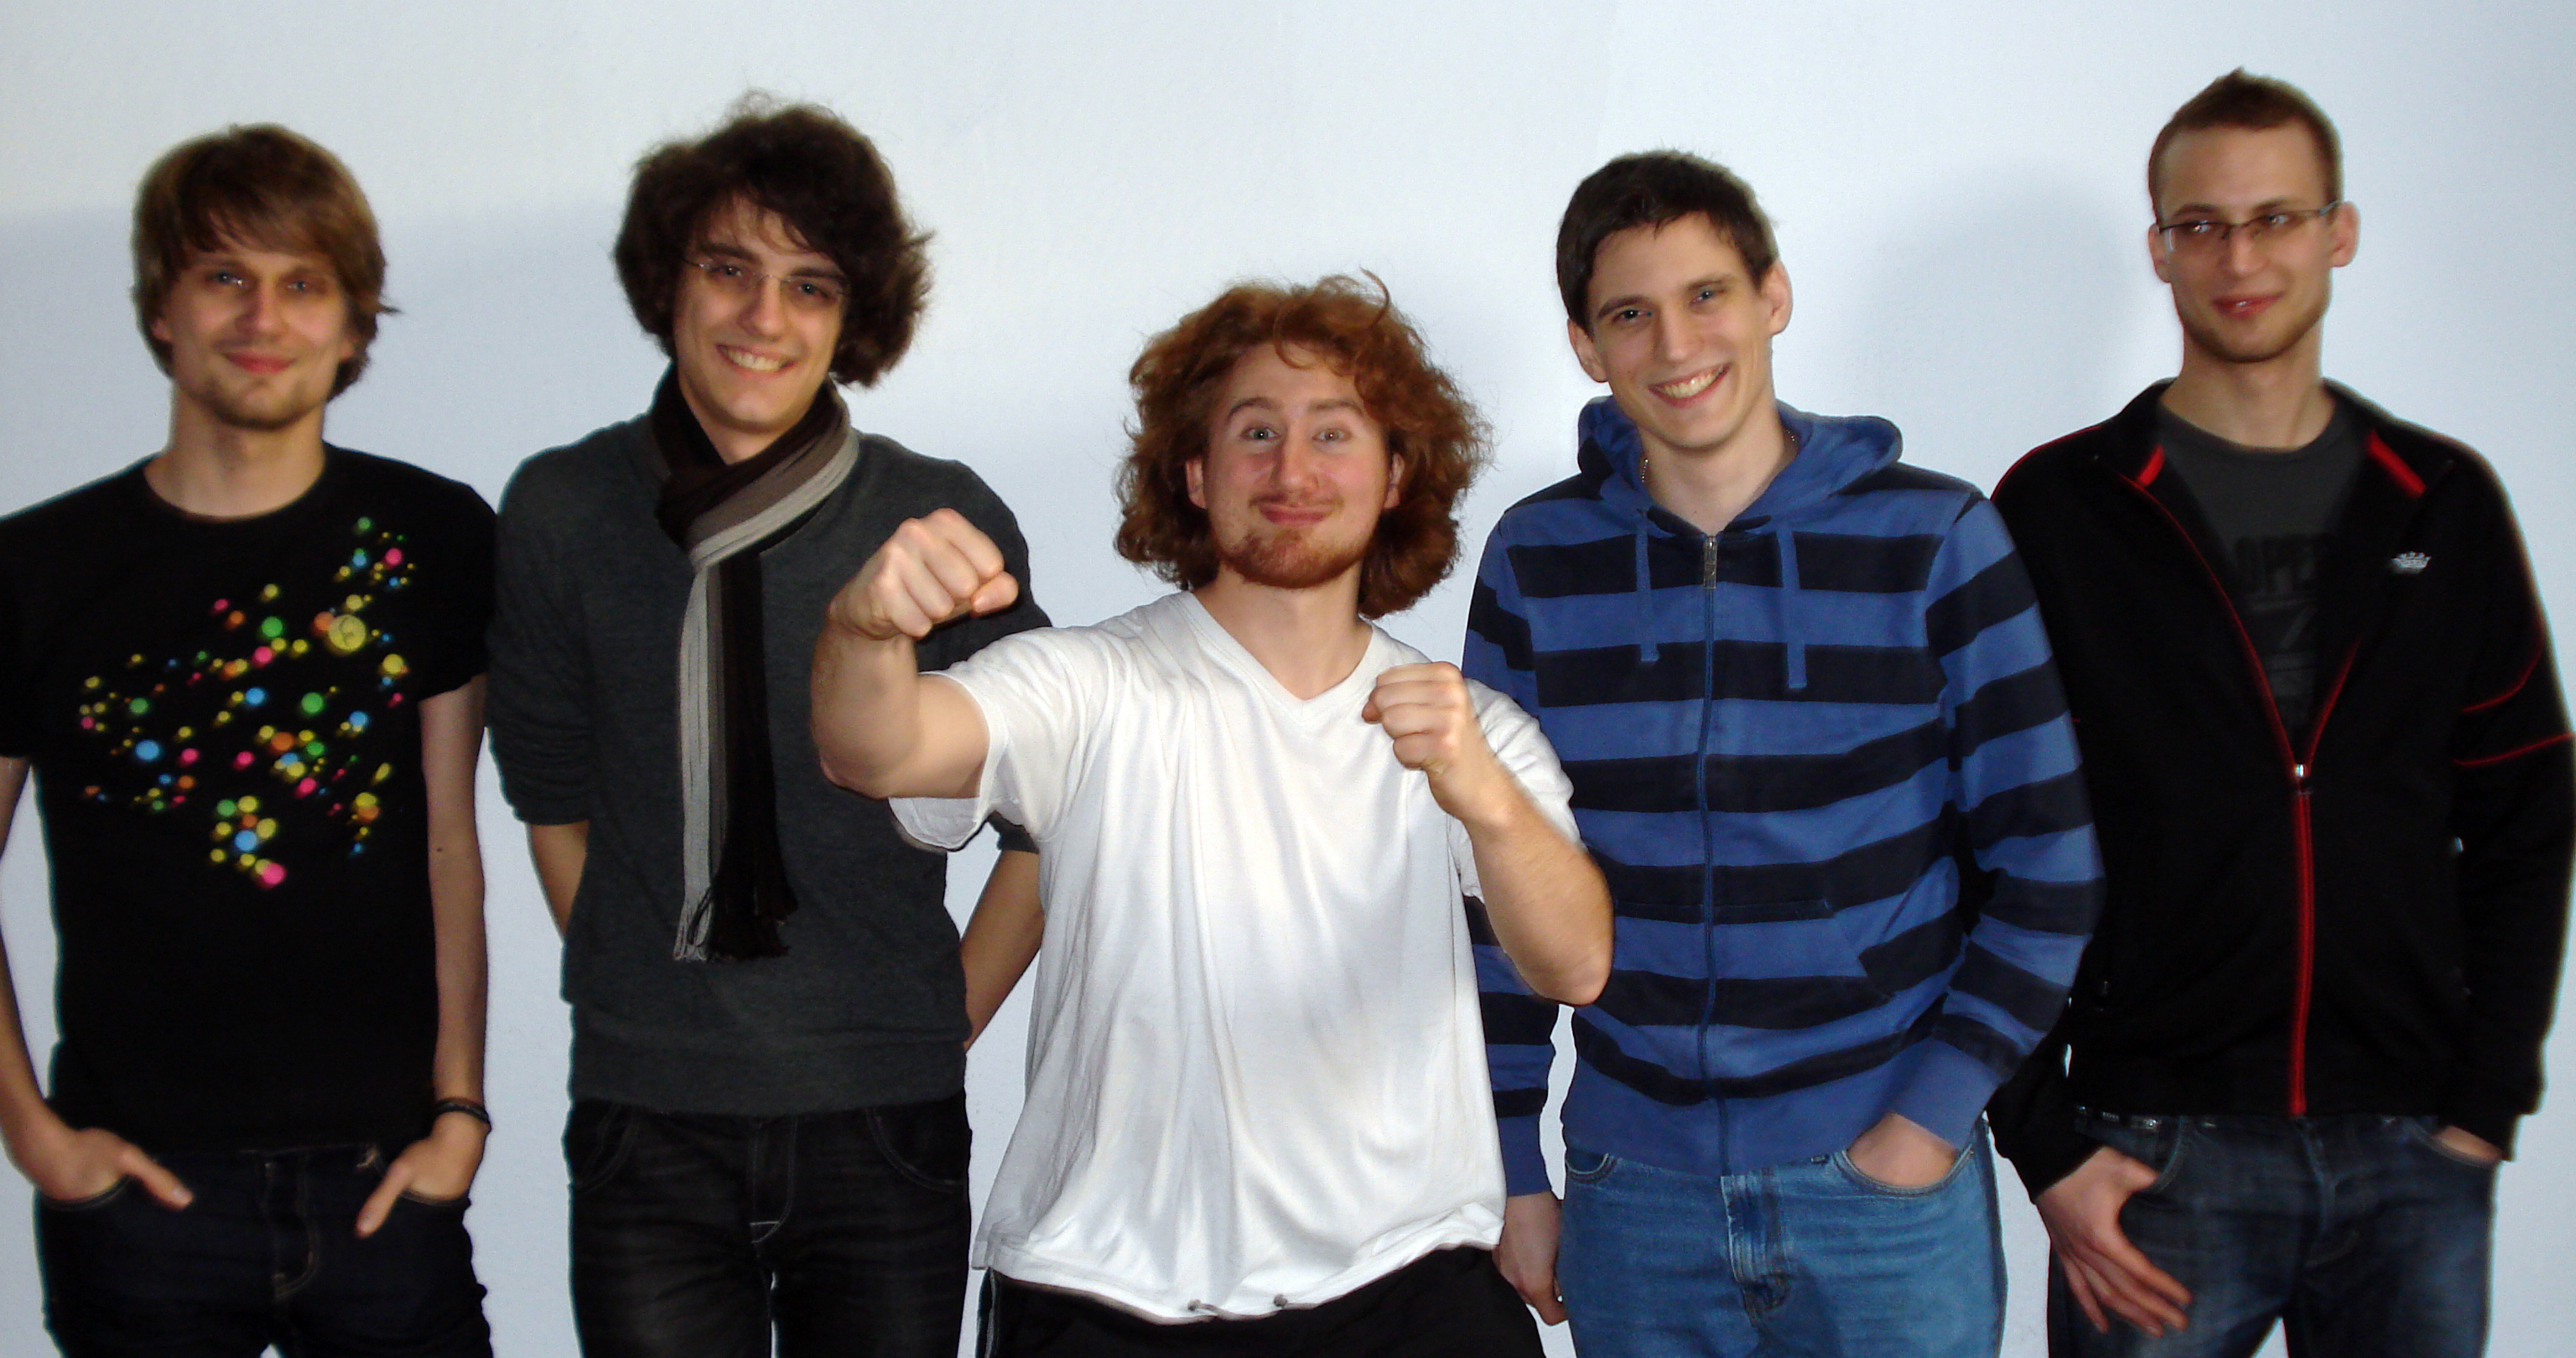
\includegraphics[width=\columnwidth]{images/team.jpg}
	\caption{\small From left to right: Andre Zoufahl, Konrad Reiche, Julian Fleischer, David Bialik, Hagen Mahnke}
	\label{fig:us}
\end{figure}
